\documentclass[12pt,aspectratio=169]{beamer}
\usepackage{pgfpages}
\usepackage{fancyvrb}
\usepackage{tikz}
\usepackage{pgfplots}
\usepackage{mdframed} %for framed boxes
\usepackage{amsthm} %for theorem formatting 
\usepackage{tcolorbox} % For colored boxes

% Include the custom theme and commands
\usepackage{/Users/posmikdc/Documents/assets/latex/beamer/beamertheme}
% Identifiers
\newcommand{\name}{Daniel C. Posmik}
\newcommand{\department}{Brown University School of Public Health, Department of Biostatistics}
\newcommand{\emailuniversity}{daniel_posmik@brown.edu}
\newcommand{\emailpersonal}{posmikdc@gmail.com}
\newcommand{\cell}{+1 224-507-4045}

% Footnote Alignment
\makeatletter % aligns multi-line footnotes properly
\renewcommand<>\beamer@framefootnotetext[1]{%
  \global\setbox\beamer@footins\vbox{%
    \hsize\framewidth
    \textwidth\hsize
    \columnwidth\hsize
    \unvbox\beamer@footins
    \reset@font\footnotesize
    \@parboxrestore
    \protected@edef\@currentlabel
         {\csname p@footnote\endcsname\@thefnmark}%
    \color@begingroup
      \uncover#2{\@makefntext{%
        \rule\z@\footnotesep\ignorespaces\parbox[t]{.9\textwidth}{#1\@finalstrut\strutbox}\vskip1sp}}%
    \color@endgroup}%
}
\makeatother

% Citations and Bibliography
\renewcommand*{\nameyeardelim}{\addcomma\addspace} % add comma between author name and year
\renewcommand{\cite}[1]{\citeauthor{#1} (\citeyear{#1})} % customize \cite to "[Author name] (Year)"
\renewcommand{\footcite}[1]{\footnote{\citeauthor{#1} (\citeyear{#1})}} % customize \footcite to "[Author name] (Year)"
%\renewcommand{\footfullcite}[1]{\footnote{\citeauthor{#1}. \citetitle{#1}. (\citeyear{#1})}} % customize \footfullcite to "[Author name]. "[Title]." ([Year])"
\renewcommand{\footfullcite}[1]{%
    \AtNextCite{\defcounter{maxnames}{2}\defcounter{minnames}{1}}%
    \footnote{\citeauthor{#1}\ifnumgreater{\value{labelname}}{2}{\space et al.}{\relax}. \citetitle{#1}. (\citeyear{#1})}%
}

% Math Abbreviations
\def\p{\mathrm{P}}
\def\Pr{\mathrm{Pr}}
\def\P{\mathbb{P}}
\def\E{\mathbb{E}}
\def\V{\mathrm{Var}}
\def\CV{\mathrm{Cov}}
\def\X{\mathfrak{X}}
\def\Sum{\sum\nolimits}
\def\Prod{\prod\nolimits}



\title{Fancy Title: \\ Followed by Some More Text}

\author{\name \inst{1} \and John Doe \inst{2} \and Don Joe \inst{2}}

\institute[shortinst]{\inst{1} \department \\ 
                      \inst{2} Another University, Another Department
}

\begin{document}

{
  % rather than use the frame options [noframenumbering,plain], we make the
  % color match, so that the indicated page numbers match PDF page numbers
  \setbeamercolor{page number in head/foot}{fg=background canvas.bg}
  \begin{frame}
    \titlepage
  \end{frame}
}

\begin{frame}{Overview}
    % Throughout your presentation, if you choose to use \section{} and \subsection{} commands, these will automatically be printed on this slide as an overview of your presentation
    \tableofcontents
\end{frame}

\section{Test1}
\begin{frame}{A slide with some bracketed text}

	\begin{itemize}
		\item Some statement\footnote{This is a footnote.} {\color{gray} [Some citation]}
		\item Another statement\footnote{This is a footnote.} {\color{gray} [Another citation]}
		\item A final statement\footnote{This is a footnote.} {\color{gray} [The last citation]}
	\end{itemize}

	\vspace{3ex}
	\begin{center}
		\scriptsize (a small note)
	\end{center}

\end{frame}

\begin{frame}{A slide title}

  \begin{itemize}
    \item A bulleted item
    \item Another item
      \begin{itemize}
        \item With sub-bullets\footnote{Test}
        \item And another, with some \textbf{bold} text
      \end{itemize}
    \item And another, at the top level, with \textit{italic} text
  \end{itemize}

\end{frame}

\section{Test2}
\begin{frame}{Blocks of Highlighted Text and Theorems}
In this slide, some important text will be \alert{highlighted} because it's important. Please, don't abuse it.

\begin{mdframed}
Test
\end{mdframed}

\begin{theorem}[Fundamental theorem of calculus]
If a function \( f \) is continuous on the closed interval \([a, b]\) and \( F \) is an antiderivative of \( f \) on \([a, b]\), then
\[ \int_a^b f(x) \, dx = F(b) - F(a). \]
\end{theorem}

\end{frame}

\begin{frame}{A slide with centered text}

  \begin{center}
    Some statement that is centered.
  \end{center}

  \vspace{2ex}
  \begin{center}
    \scriptsize (a small note)
  \end{center}

\end{frame}

\begin{frame}{A slide with some text and a link}

  \begin{itemize}
    \item This slide has some text along with a link
      \begin{itemize}
        \item \textbf{Some bold text}: followed by an explanation
        \item \textbf{More bold text}: followed by more text
      \end{itemize}
    \item Another bullet, with sub-bullets
      \begin{itemize}
        \item A sub-bullet
        \item Another sub-bullet, with more text
      \end{itemize}
  \end{itemize}

  \vspace{2ex}
  \begin{center}
    \color{blue} \href{https://github.com/anishathalye/auriga}{github.com/anishathalye/auriga}
  \end{center}

\end{frame}

\begin{frame}[fragile]{A slide with some code}

	\begin{columns}
		\begin{column}{0.5\linewidth}
			\footnotesize
			\begin{Verbatim}[commandchars=\\\{\}]
/* some code */
def foo(x):
  return x**0.5 + 2*x

\color{blue}/* some can be highlighted */
\color{blue}foo(3)
      \end{Verbatim}
    \end{column}
    \begin{column}{0.5\linewidth}
      {\color{red} Some explanatory text, in red, with some \texttt{monospace} text.}
      There might be some math, too:

      $$\sqrt{x} + 2x + \sum_{i=1}^{N} x_i^2 + \int_{-\infty}^{+\infty}x~dx$$
    \end{column}
  \end{columns}

\end{frame}

\begin{frame}{A 50-50 split slide}

  \begin{columns}
    \begin{column}{0.5\linewidth}
      \begin{itemize}
        \item This side has a bullet
        \item And another bullet, with text that wraps if it's long
      \end{itemize}
    \end{column}
    \begin{column}{0.5\linewidth}
      \begin{figure}
        \centering
        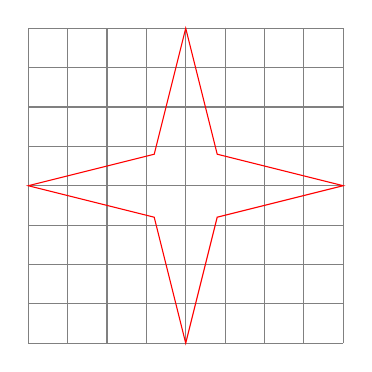
\begin{tikzpicture}[scale=2]
          \draw[step=0.25cm,color=gray] (-1,-1) grid (1,1);
          \draw[color=red] (1,0) -- (0.2,0.2) -- (0,1) -- (-0.2,0.2) -- (-1,0)
          -- (-0.2,-0.2) -- (0,-1) -- (0.2,-0.2) -- cycle;
        \end{tikzpicture}
        \caption{A figure caption}
      \end{figure}
    \end{column}
  \end{columns}

\end{frame}

\end{document}

